\documentclass[a4paper]{tufte-handout}

\usepackage[utf8]{inputenc}
\usepackage{tikz}
\usepackage{hyperref}
\usepackage{amsmath}
\usepackage{amssymb}
\usepackage{listings}

\lstdefinestyle{style}{
    basicstyle=\ttfamily,
    numbers=left,
    numberstyle=\small\ttfamily,
    captionpos=b,
    frame=tlrb,
}
\lstset{style=style}

\title{CP Course Notes}

\begin{document}
\maketitle
\section{Parallel Architectures}

\subsection{Flynn's Taxonomy}

\subsubsection{Instruction Level}
\begin{itemize}
    \item Single Instruction (SI) - System in which all processors execute the same instruction
    \item Multiple Instruction (MI) - System in which different processors execute may execute different instructions
\end{itemize}

\subsubsection{Data Level}
\begin{itemize}
    \item Single Data (SD) - System in which all processors operate on the same data
    \item Multiple Data (MD) - System in which different processors may operate on different data
\end{itemize}

\subsubsection{Existing Architectures}

\begin{figure}[h]
    \centering
    \begin{tabular}{c | c | c}
           & SD   & MD   \\
        \hline
        SI & SISD & SIMD \\
        \hline
        MI & MISD & MIMD \\
    \end{tabular}
    \caption{Possible processor architectures. MISD is the exception.}
    \label{fig:flynn}
\end{figure}

\paragraph{SISD}
The classic Von Neumann architecture, present in serial processors
\begin{figure}[h]
    \centering
    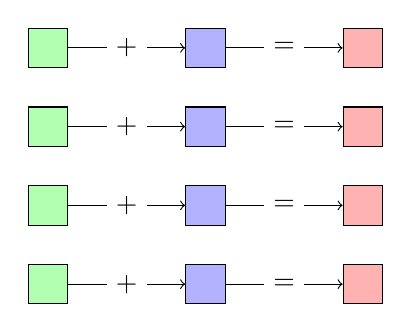
\begin{tikzpicture}

        \foreach \y in {0,..., 3}
            {
                \node[name=1_\y, draw, rectangle, minimum size=0.5cm, fill=green!30] at (0, \y) {};
                \node[name=2_\y, draw, rectangle, minimum size=0.5cm, fill=blue!30] at (2, \y) {};
                \node[name=3_\y, draw, rectangle, minimum size=0.5cm, fill=red!30] at (4, \y) {};
                \draw[->] (1_\y) -- node [fill=white] {$+$} (2_\y);
                \draw[->] (2_\y) -- node [fill=white] {$=$} (3_\y);
            }
    \end{tikzpicture}
    \caption{SISD Processing Example. One instruction is applied to each data item.}
    \label{}
\end{figure}

\paragraph{SIMD}
The data is divided among the processors and each item is subjected to the same sequence of instructions. Present in modern CPUs through Advanced Vector Extensions (AVX), as well as GPUs.
\begin{figure}[h]
    \centering
    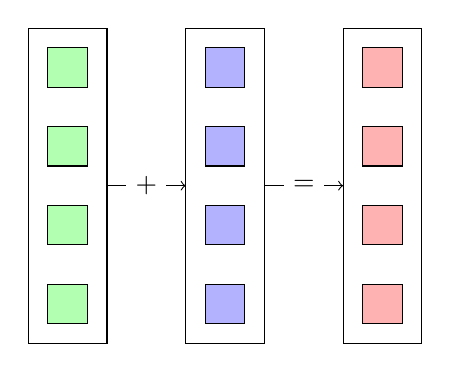
\begin{tikzpicture}

        \foreach \y in {0,..., 3}
            {
                \node[name=1_\y, draw, rectangle, minimum size=0.5cm, fill=green!30] at (0, \y) {};
                \node[name=2_\y, draw, rectangle, minimum size=0.5cm, fill=blue!30] at (2, \y) {};
                \node[name=3_\y, draw, rectangle, minimum size=0.5cm, fill=red!30] at (4, \y) {};
            }
        \draw (-.5, -.5) rectangle (.5, 3.5);
        \draw (1.5, -.5) rectangle (2.5, 3.5);
        \draw (3.5, -.5) rectangle (4.5, 3.5);
        \draw[->] (.5, 1.5) --  node[fill=white] {$+$} (1.5, 1.5);
        \draw[->] (2.5, 1.5) -- node[fill=white] {$=$} (3.5, 1.5);
    \end{tikzpicture}
    \caption{SIMD Processing Example. One instruction is applied to a block of data items.}
    \label{}
\end{figure}

\paragraph{MISD}
Possible to envision as a pipeline at most, since it is not possible for multiple instructions to execute at the same time over the same data item.

\paragraph{MIMD}
Collection of autonomous processors executing independent programs, such as a distributed network or cluster.
MIMD architectures can be categorized under four designations, each with different purposes, some of these architectures may be composed to form more complex systems.

\begin{figure}[h]
    \centering
    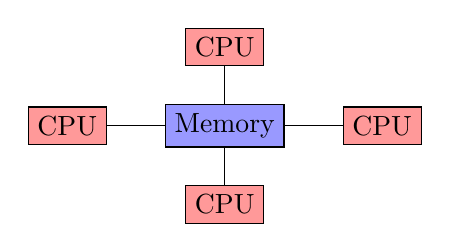
\begin{tikzpicture}
        % \draw (0, 0) grid (4,2);
        \node[draw, fill=blue!40, name=memory] at (2, 1) {Memory};
        \node[draw, fill=red!40, name=cpu_1] at (0, 1) {CPU};
        \node[draw, fill=red!40, name=cpu_2] at (2, 2) {CPU};
        \node[draw, fill=red!40, name=cpu_3] at (2, 0) {CPU};
        \node[draw, fill=red!40, name=cpu_4] at (4, 1) {CPU};
        \draw[-] (cpu_1) -- (memory);
        \draw[-] (cpu_2) -- (memory);
        \draw[-] (cpu_3) -- (memory);
        \draw[-] (cpu_4) -- (memory);
    \end{tikzpicture}
    \caption{Uniform Memory Access (UMA). This architecture suffers from the need of synchronization among memory accesses. We can picture this as several CPUs accessing common RAM.}
    \label{fig:sm:uma}
\end{figure}

% \begin{figure}[h]
%     \centering
%     \begin{tikzpicture}
%         \draw (-5, -2) grid (5, 2);
%         \draw (-4.5, .5) rectangle (-.5, 1.5);
%         \draw [-] (-2.5, .5) -- (-2.5, 1.5);
%     \end{tikzpicture}
%     \caption{Non-Uniform Memory Access (NUMA). Common in distributed architectures.}
%     \label{fig:sm:numa}
% \end{figure}

\subsection{Software Taxonomies}

Applying Flynn's taxonomy to software we observe the following patterns.

\begin{itemize}
    \item Data Parallel (SIMD) - Parallelism that is a result of identical operations applied concurrently on different data items. This approach is difficult to apply to complex problems.
    \item Single Program, Multiple Data (SPMD) - A single program is run across multiple processing units (computers, processors, threads). Processing units execute the same code but do not work in lock-step.
\end{itemize}

\subsection{Memory}

Memory can be split into shared memory or distributed memory.

\subsubsection{Shared Memory}

Shared memory represents a global memory space, it is accessed by every processor.
Each processor has a local cache (L1, L2, L3) which keep portions of the memory for faster access.
The L1 and L2 caches are available at a core level while the L3 cache is shared among cores.

Shared memory is easier to program with, several frameworks are available (e.g. OpenMP, OpenACC).
Low latency for data sharing between tasks.
However the programmer is responsible for synchronization, furthermore the memory access is non-uniform (NUMA) and accesses to global memory (RAM) can be a bottleneck.

\subsubsection{Distributed Memory}

Memory is shared between processes using messages (OpenMPI), this allows to exploit distributed computing architectures in a cost effective way.

Memory scales based on the number of processors and the access to local memory is fast.

This approach however is complex due to difficulties in programming communication effectively and data structures may be difficult to distribute.
\chapter{Parallel Performance}


\section{Performance}

In computing performance can be defined by two factors,
computational requirements or resources.
Computational requirements can be thought of "what needs to be done?", or efficacy,
and computational resources can be thought in terms of "how much will it cost?", or efficiency.

\begin{equation}
    \mathnormal{Performace} \sim \frac{1}{\mathnormal{Resources~for~solution}}
\end{equation}

\subsection{Expectations}

In a scenario where we have $p$ processors and each processor is rated at $f$ MFLOP, should we see $f \times p$ MFLOPS performance?

The answer is not as simple as "yes".
Several causes may affect performance, while causes may interact with each other,
they need to be understood separately.

\subsection{Embarrassingly Parallel Computations}

Or for short EPCs, are computations that can be trivially divided into several independent parts able to be executed simultaneously.
For \textit{truly} EPCs there should be no interaction between processes, while in \textit{nearly} EPCs the input and output is required to be distributed and combined in some way.

EPCs have potential to achieve maximal speedups in parallel platforms.


\subsection{Scalability}
As previously discussed the performance of a parallel solution is subjected to several factors, namely scalability.
Scalability is the ability of a parallel algorithm of achieving performance gains proportional to the number of processors and the size of the problem.

\paragraph{Evaluation}

To evaluate scalability we can start from the following metrics.

\begin{itemize}
    \item Sequential Runtime ($T_{seq}$) which is a function of problem size and architecture.
    \item Parallel Runtime ($T_{par}$) which is a function of problem size and parallel architecture, that is the number of processors used in execution.
\end{itemize}

With that in mind we can define the speedup $S_p$ as \autoref{eq:speedup},
efficiency $E_p$ as \autoref{eq:efficiency}
and finally the cost $C_p$ as \autoref{eq:cost},
where $p$ is the number of available processors and $T_p$ is the execution time on a $p$ processor system\sidenote{A parallel algorithm is cost-optimal if $C_p = T_1$ or equivalently $E_p = 1$}.

\begin{equation}\label{eq:speedup}
    S_p = \frac{T_1}{T_p}
\end{equation}

\begin{equation}\label{eq:efficiency}
    E_p = \frac{S_p}{p}
\end{equation}

\begin{equation}\label{eq:cost}
    C_p = p \times T_p
\end{equation}
\section{Amdahl's Law}

Amdahl's law fixes the problem size and varies the number of processors,
hence the denomination of Fixed Size Speedup.
The law relates at the reduction of the execution time.
Let $f$ be the sequential fraction of a program, $1-f$ is the part that can be parallelized.

\begin{equation}
    \begin{split}
        S_p & \le \frac{T_1}{T_p} = \frac{T_1}{(f \cdot T_1) + \frac{(1_f)T_1}{p}}\\
        S_p & \le \frac{1}{f + \frac{1-f}{p}}\\
        S_{p \leadsto \infty} & \le \frac{1}{f}
    \end{split}
\end{equation}

\paragraph{Scalability}
When considering scalability, Amdahl's law refers to the abillity of a parallel algorithm to achieve performance gains proportional to the number of processors and the size of the problem.

\paragraph{Application}

Amdahl's law is applicable under the following circumstances:
\begin{itemize}
    \item When the problem size is fixed.
    \item Strong scaling ($p\rightarrow\infty$, $S_p = S_{\infty} \rightarrow \frac{1}{f}$).
    \item Speedup bound is determined by the degree of sequential execution time in the computation.
\end{itemize}

\paragraph{Example}

If $90\%$ of the computation can be parallelized, what is the maximum speedup achievable using 8 processors?

We first calculate the sequential part of the program:

\begin{equation*}
    \begin{split}
        0.9 & = 1 - f\\
        f & = 0.1
    \end{split}
\end{equation*}

And then apply Amdahl's law:

\begin{equation*}
    \begin{split}
        S_8 & \le \frac{1}{0.1 + \frac{1-0.1}{8}}\\
        S_8 & \le 4.7
    \end{split}
\end{equation*}

\subsection{Gustafson-Barsis’ Law}

Also denominated as Scaled Speedup, it is interested in larger problems when scaling.
In other words, for the same time, how much more work can we do?

Considering $a$ the non-parallelizable part and $b$ as the parallelizable part,
we calculate $T_P$, for $P$ processors, as follows:
\begin{equation}
    \begin{split}
        T_P & = a + P \cdot b\\
        T_1 & = a + 1 \cdot b\\
        & = a + b
    \end{split}
\end{equation}

Given that the wall-clock execution time is always the same,
the scaled speedup is calculated on the volume of data processed.

\begin{equation}
    \begin{split}
        S_P & \le \frac{T_P}{T_1}\\
        & \le \frac{a + P \cdot b}{a + b}
    \end{split}
\end{equation}

Consider $\alpha = \frac{a}{a+b}$ as the sequential fraction of the parallel execution time.
We can then define the scaled speedup as follows:

\begin{equation}
    \begin{split}
        S_P & \le \alpha + P \cdot (1-\alpha)\\
        & \le P - \alpha \cdot (P-1)
    \end{split}
\end{equation}

\paragraph{Scalability}
The ability of a parallel algorithm to achieve performance gains proportional to the number of processors and the size of the problem.

\paragraph{Application}

The Gustafson’s law applies under the following scenarios:
\begin{itemize}
    \item When the problem size can increase.
    \item When the number of processors increases.
    \item Speedup function include the number of processors.
    \item Can maintain or increase parallel efficiency as the problem scales.
\end{itemize}

\paragraph{Example} An application executing on $64$ processors spends $5\%$ of the total time on non-parallelizable computations.
What is the scaled speedup?

\begin{equation}
    \begin{split}
        S_64 & \le P - \alpha \cdot (P-1)\\
        & \le 64 - 0.05 \cdot (64 - 1)\\
        & \le 60.85
    \end{split}
\end{equation}

\subsection{Computational DAG}

A parallel program maybe be represented as a directed acyclic graph (DAG),
this graph has several properties, such as the span,
which can be used to evaluate the potential performance of an algorithm.

\begin{figure}[h]
    \centering
    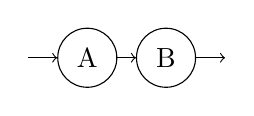
\begin{tikzpicture}
        \node[name=a, draw, circle, minimum size=0.75cm] at (0,0) {A};
        \node[name=b, draw, circle, minimum size=0.75cm] at (1,0) {B};
        \draw[->] (-.75, 0) -- (a);
        \draw[->] (a) -- (b);
        \draw[->] (b) -- (1.75,0);
    \end{tikzpicture}
    \caption{Serial Composition}
    \label{fig:dag:serial}
\end{figure}[h]


\begin{figure}[h]
    \centering
    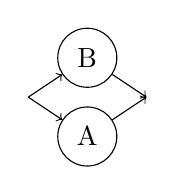
\begin{tikzpicture}
        \node[name=a, draw, circle, minimum size=0.75cm] at (0,0) {A};
        \node[name=b, draw, circle, minimum size=0.75cm] at (0,1) {B};
        \draw[->] (-.75, 0.5) -- (a);
        \draw[->] (-.75, 0.5) -- (b);
        \draw[->] (a) -- (.75, 0.5);
        \draw[->] (b) -- (.75, 0.5);
    \end{tikzpicture}
    \caption{Parallel Composition}
    \label{fig:dag:parallel}
\end{figure}[h]

\paragraph{Work}

The total number of tasks of the graph is called \textit{work},
this is equivalent to running the algorithm with a single processing unit ($T_1$).

\begin{equation}\label{eq:work_law}
    T_p \ge \frac{T_1}{P}
\end{equation}

The work is equal whether considering $T_1$ or $T_P$,
that is:

\begin{equation}
    T_1 (A \cup B) = T_1(A) + T_1(B)
\end{equation}

\paragraph{Span}

The span, or the critical-path length, is the minimum of sequential steps the algorithm must execute.

\begin{equation}\label{eq:span_law}
    T_p \ge T_{\infty}
\end{equation}

The span is different when comparing $T_1$ and $T_P$.

\begin{equation}
    \begin{split}
        T_{\infty} (A \cup B) & = T_{\infty}(A) + T_{\infty}(B)\\
        T_{\infty} (A \cup B) & = max\{T_{\infty}(A), T_{\infty}(B)\}\\
    \end{split}
\end{equation}

\subsubsection{Speedup}

The speedup on $P$ processors is given by:

\begin{equation}
    \frac{T_1}{T_P}
\end{equation}

If $\frac{T_1}{T_P} = P$ we have \textit{linear} speedup.
When $\frac{T_1}{T_P} \ge P$ we have \textit{superlinear} speedup,
this however is not possible due to the work law (\autoref{eq:work_law}).

\subsubsection{Parallelism}

Parallelism can be defined as the average amount of work per step along the span, that is:

\begin{equation}
    \frac{T_1}{T_\infty}
\end{equation}

\subsubsection{Work-Span Model}

Considers a greedy scheduler, that is,
no worker is idle while there are tasks to execute.

\begin{itemize}
    \item $T_P$ - running time with $P$ workers.
    \item $T_1$ - running time with 1 worker, serial execution.
    \item $T_\infty$ - the time taken along the critical path.
\end{itemize}

The critical path is the sequence of tasks that has the longest execution time.

\paragraph{Lower-Bound}
A lower-bound can be calculated with the following formula:

\begin{equation}
    \mathnormal{max}\left(\frac{T_1}{P}, T_\infty\right) \le T_P
\end{equation}

\paragraph{Upper-Bound}

\begin{equation}
    T_P \le \frac{T_1 - T_\infty}{P + T_\infty}
\end{equation}
\section{Parallel Programming}

Parallel programs often start as sequential programs.
This approach has the advantage of having a previous codebase to validate the new approach,
furthermore it is easier to start with a sequential approach given the ease of programming and debugging.

To parallelize a program we first have to evaluate if it is worth the effort,
to do so we first identify the hotspots with a profiler.

The parallelization process starts with the hotspots,
applying small changes with testing in-between.

\subsection{Finding Concurrency}

The first step in parallelizing a candidate program is to find concurrency,
in other words, we have to find tasks that can be executed at the same time.

To do so, we need to consider flexibility, efficiency and simplicity.

\subsubsection{Task Decomposition Guidelines}

\paragraph{Flexibility}
The program design should afford flexibility in the number and size of the tasks generated.

\paragraph{Efficiency}
Tasks should have enough work as to amortize the cost of creating and managing them.
furthermore, they should be sufficiently independent so that managing dependencies does not become the bottleneck.

\paragraph{Simplicity}
The code must remain as simple and readable as possible so as to be debuggable and quick to understand and modify.

\subsubsection{Data Decomposition Guidelines}

Often implied by task decomposition,
data decomposition is a good starting point when the main computation is organized around manipulation of large data structures
or similar operations are applied to different parts of the data structure.

\paragraph{Flexibility}
The size and number of data chunks should support a wide range of executions.

\paragraph{Efficiency}
Data chunks should generate considerable amounts of work to minimize the communication and management impact.

\paragraph{Simplicity}
Complex data compositions can get difficult to manage and debug.

\subsection{Algorithmic Structure Design Space}

The high level approach of an algorithm can be split in to three possibilities, all approaches can then be split into two sub approaches,
the linear or recursive approach.

\begin{itemize}
    \item Organize by Tasks - the linear approach to this problem is to make use of task parallelism, the recursive approach is through divide and conquer.
    \item Organize by Data Decomposition - the linear approach of data decomposition is by making use of geometric decomposition (arrays), the recursive approach is through recursive data structures.
    \item Organize by Data Flow - the linear solution is to make use of the pipeline pattern, the recursive approach is based on event coordination.
\end{itemize}

\subsection{Implementation Environment}

\subsubsection{Program Structures}

\paragraph{Single Program Multiple Data}
In the SMPD approach all tasks execute the same program in parallel but each has its own set of data.

\paragraph{Master/Worker Pattern}
The master/worker is works by having a thread distribute work amongst the others,
the workers execute concurrently and each worker takes tasks from the bag of tasks.
It is suited for embarrassingly parallel problems.

\paragraph{Loop Parallelism Pattern}
This pattern exploits the iterative nature of some programs by parallelizing the execution of loop iterations.
This requires the loop not to have dependencies among iterations.

\paragraph{Fork/Join Pattern}
A main task forks off some number of other tasks that then continue in parallel, the main task then waits for completion before moving on.

\paragraph{Pipeline Pattern}
Tasks are applied in sequence to data.

\chapter{Parallel Patterns}

A parallel pattern is a recurring combination of task distribution and data access that solves a specific design problem in parallel algorithm design.

\section{Nesting Pattern}

Nesting is the ability to hierarchically compose patterns.
This pattern appears in both serial and parallel algorithms.

It is a compositional pattern, allowing other patterns to be composed in such way that task blocks can be replaced with another pattern.

\section{Control Patterns}

\subsection{Serial Control Patterns}

Structured serial programming is based on following patterns.

\paragraph{Sequence}
Ordered list of tasks that are executed in a specific order.

\paragraph{Selection}
Condition $c$ is first evaluated.
Either task $a$ or $b$ is executed depending on the true or false result of $c$.

\paragraph{Iteration}
Condition $c$ is evaluated, if it is true $a$ is evaluated again,
afterwards $c$ is evaluated again.
This repeats until $c$ is false.

\paragraph{Recursion}
Dynamic form of nesting allowing functions to call themselves.

\subsection{Parallel Control Patterns}
Parallel control patterns extend serial control patterns.
Each parallel control pattern is related to at least one serial control pattern.

\paragraph{Fork-Join}
Allows control flow to fork into multiple parallel flows, then rejoin later.

\paragraph{Map}
Performs a function over every element of a collection, it replicates a serial iteration pattern.

\paragraph{Stencil}
Elemental function accesses a set of "neighbors", stencil is a generalization of map.

\paragraph{Reduction}
Combines every element of a collection using an associative "combiner function".

\paragraph{Scan}
Computes all partial reductions of a collection.
For every output in a collection, a reduction of the input up to that point is computed.

\paragraph{Recurrence}
More complex version of map, where loop iterations can depend on one another.

\section{Data Management Patterns}

\subsection{Serial Data Management Patterns}

\paragraph{Random Read \& Write}
Memory locations indexed with addresses, used with pointers.
Aliasing can cause problems when parallelizing the code.

\paragraph{Stack Allocation}
Useful for dynamically allocate data in LIFO manner.
It preserves locality and when parallelized, since each threads gets its own stack thread locality is preserved.

\paragraph{Heap Allocation}
Useful when data cannot be allocated in LIFO manner.
Slower and more complex when compared with stack allocations.
A parallelized allocator should be used when allocating memory in parallel.

\paragraph{Objects}
Objects are language constructs to associate data with code to manipulate and manage that data.

\subsection{Parallel Data Management Patterns}

\paragraph{Pack}
Used to eliminate unused space in a collection.

\paragraph{Pipeline}
Connects tasks in a producer-consumer manner.

\paragraph{Geometric Decomposition}
Arranges data into subcollections.
Overlapping and non-overlapping compositions are possible.

\paragraph{Gather}
Reads a collection of data given a collection of indices.

\paragraph{Scatter}
The inverse of gather, given a collection of indices, it writes to such indices.
\chapter{Parallel Models \& Dependencies}

\section{Parallelism, Correctness \& Dependencies}

Parallel execution shall always be constrained by the sequence of operations needed to be performed for a correct result.
Such execution must address control, data and system dependencies.

A \textit{dependency} arises when one operation depends on an earlier operation to complete and produce a result before this later operation can be performed.

\subsection{Sequential Consistency}

Sequential consistency implies that the execution of two statements do not interfere with each other, meaning their running order is irrelevant.
This means that the statements are \textit{independent},
if the order of execution affects the computation outcome they are deemed \textit{dependent}.

\subsection{Dependencies}

\paragraph{True Dependency}
A statement $S2$ has a true dependency on statement $S1$ if and only if $S2$ reads a value written by $S1$.
This dependency is also known as Read After Write (RAW).

Formally we can describe a true dependency as follows:
\begin{equation*}
    out(S_1) \cap in(S_2) \neq \emptyset
\end{equation*}

\paragraph{Anti-Dependency}
A statement $S2$ has an anti-dependency in statement $S1$ if and only if $S2$ writes a value read by $S1$.
This dependency is also known as Write After Read (WAR).

Formally we can describe an anti-dependency as follows:
\begin{equation*}
    in(S_1) \cap out(S_2) \neq \emptyset
\end{equation*}

\paragraph{Output Dependency}
A statement $S2$ has an output dependency on $S1$ if and only if $S2$ writes a variable written by $S1$.
This dependency is also known as Write After Write (WAW).

Formally we can describe an output dependency as follows:
\begin{equation*}
    out(S_1) \cap out(S_2) \neq \emptyset
\end{equation*}

\paragraph{Loop-Carried Dependencies}
A loop-carried dependency is a dependency between two statement instances in two different loop iterations.
\chapter{Synchronization}

\section{Algorithms, Programs \& Processes}

\paragraph{Sequential Algorithm}
A sequential algorithm is a forma description of the behavior of a sequential state machine.

\paragraph{Concurrent Algorithm}
The description of a set of sequential states machines that cooperate through a communication medium is called a concurrent algorithm.

\paragraph{Program}
When the algorithm is written in a specific programming language.

\paragraph{Process}
The running instance of an algorithm and thus of a program as well.

\section{Process Synchronization}
Process synchronization occurs when the progress of one or several processes depends on the behavior of other processes.
Two types of process interaction require synchronization, competition and cooperation.

\subsection{Competition}
Competition occurs when processes compete to execute some statements and only one process at a time is allowed to execute them.

\subsection{Cooperation}
Cooperation occurs when one process can only progress after some event on another process.

\paragraph{Barrier}
A barrier is a set of control points, one per process involved in the barrier,
such that each process is allowed to pass its control point only when all other processes have attained their own control points.
From an operation point of view, each process has to stop until all other processes have arrived at their control point.

\subsection{The Producer/Consumer Problem}

In the producer/consumer problem we have a producer that loops forever, producing data items,
and a consumer that loops forever, consuming said data items.

It is required to ensure that,
only produced data items are consumed and each produced item is consumed exactly once.

\paragraph{Synchronization Barrier}
One approach to the problem consists in using a synchronization barrier to ensure that only when a data item is produced the consumer is able to consume it.
While this approach works it is far from efficient.

\paragraph{Shared Buffer}
The buffer has size greater than 1 and the underlying structure can be a queue or a circular array.
Whenever the producer has a new item, it adds the item at the end of the structure,
the consumer then withdraws items from the head of the structure.

This way the producer only waits whenever the structure is full,
the consumer will only wait whenever the structure is empty.

\subsection{The Mutual Exclusion Problem}

\paragraph{Critical Section}
A part (or several parts) that are required to be executed by a single process at a time.

\paragraph{Solution}
We are required to provide an entry algorithm as well as an exit algorithm,
these are used to respectively enter and exit the critical section,
ensuring that the critical section is only executed once.

\paragraph{Mutual Exclusion Definition}
The mutual exclusion problem consists in implementing the operations to acquire and release a mutex
in such a way that the following properties are always satisfied:

\begin{itemize}
    \item \textbf{Mutual Exclusion} - at most one process at a time executes the critical section code.
    \item \textbf{Starvation-Freedom} - for any process $p$ each invocation of \texttt{acquire\_mutex} $p$ eventually terminates.
\end{itemize}
\chapter{Concurrency Errors}

\subsection{Data Races}
Code is supposed to be executed atomically since there are multiple dependent instructions manipulating the same data.
This creates the possibility to several possible interleavings.

\begin{lstlisting}[caption=Deposit Operation.]{}
void Bank::Deposit(int amount)
{
  int balance = getBalance();
  setBalance(balance + amount);
}
\end{lstlisting}

\begin{lstlisting}[caption=Withdraw Operation.]{}
void Bank::Withdraw()
{
  int balance = getBalance();
  setBalance(balance - amount);
}
\end{lstlisting}

As we can see in the above example,
if the code is run in different threads the withdraw may not be reflected on the final balance,
this happens because a thread (Thread $1$) may read the balance,
then the other thread (Thread $2$) will update it,
when Thread $1$ continues the balance value it has is now outdated.

\subsubsection{Data Race Detection}

Data race detection may be executed by static or dynamic analysis.
Static analysis depends on compiler features and may report false positives.
Dynamic analysis happens at runtime, all reported data races, are data races.

\paragraph{Happens-Before Algorithm}
The Happens-Before algorithm defines a partial order for events in a set of concurrent threads.
In a single thread, happens-before reflects the temporary order of event occurrence.
Between threads, $A$ happens before $B$ if $A$ is an unlock access in one threads
and $B$ is a lock access in a different thread\footnote{Data races between threads are possible if accesses to shared variables are not ordered.}.

\begin{equation}
  \mathnormal{if}\left(a = \mathtt{unlock(mu)} \wedge b = \mathtt{lock(mu)}\right) \Rightarrow a \rightarrow b
\end{equation}

\paragraph{Lock-Set Algorithm}
The algorithm may fail and the program still be data race free (false positives),
this happens since the algorithm check a sufficient condition for data-race freedom.
This algorithm does not check for data races but rather for a consistent lock discipline.
The algorithm defines two data structures, \texttt{LocksHeld(t)}, the set of locks currently held by the thread $t$ and
\texttt{LockSet(x)}, the set of locks that could potentially be protecting variable $x$.
\begin{itemize}
  \item When thread $t$ acquires lock $l$ we have:$$\mathtt{LocksHeld(t)} = \mathtt{LocksHeld(t)} \cup \{l\}$$
  \item When thread $t$ releases lock $l$ we have:$$\mathtt{LocksHeld(t)} = \mathtt{LocksHeld(t)} \setminus \{l\}$$
  \item When thread $t$ accesses location $x$ we have:$$\mathtt{LockSet(x)} = \mathtt{LockSet(x)} \cap \mathtt{LocksHeld(t)}$$
\end{itemize}
A data race is detected if \texttt{LockSet(x)} becomes empty.
\subsection{High-Level Data Races}

Also known as high-level atomicity violations.
This happens when seemingly atomic code has interleavings that lead to a data race.

\begin{lstlisting}[caption={Class \texttt{Pair} definition, notice the synchronized methods.}]
class Pair {
  synchronized int getX() {
    return pair.x:
  }

  synchronized int getY() {
    return pair.y:
  }

  synchronized void setPair(
    int x,
    int y
  ) {
    this.x = x;
    this.y = y;
  }

  boolean areEqual() {
    int x = this.getX(); // synchronized
    int y = this.getY(); // synchronized
    return x == y;
  }
}
\end{lstlisting}

Seemingly the methods are well synchronized,
however if a thread calls \texttt{areEqual},
it is possible for the pair class to be changed between \texttt{get} calls,
running an interleaving like the following.

\begin{lstlisting}[caption={Possible incorrect interleaving. Assuming \texttt{y != y'}.}]
getX();
setPair(x', y');
getY(); // y is now y'
\end{lstlisting}

\subsubsection{Stale-Value Errors}

Stale-Value errors are caused by the privatization of data.

\begin{lstlisting}[caption={Stale-Value error example.}]
void setYToXTimesTwo() {
  int x = getX();
  setY(2 * x); // x may have changed
}

@Atomic
synchronized int getX() {
  return x;
}

@Atomic
synchronized int setY(int y) {
  this.y = y;
}
\end{lstlisting}

\subsubsection{Detecting High-Level Data Races}

A view of an atomic block $B$, named $V(B)$, is the set of variables accessed inside the atomic code block $B$.
We can define a \textit{read view} of $B$ as $V_{R}(B)$ as the set of variables read inside the atomic code block $B$.
Analogously the \textit{write view} of $B$, $V_{W}(B)$ is the set of variables written inside the atomic code block $B$.

\begin{lstlisting}[caption={
  The \texttt{getX} has the read view $V_{R}(\mathtt{getX}) = \{\mathtt{x}\}$ and the write view $V_{W}(\mathtt{getX}) = \{\}$.
}]
public int getX() {
  return this.x;
}
\end{lstlisting}

\paragraph{Direct Correlation}
There is a direct correlation between a read variable $x$ and a written variable $y$ if in the dependency graph $D$ there is a path from $x$ to $y$.

\paragraph{Common Correlation}
There is a common correlation between read variables $x$ and $y$ if,
in a dependency graph $D$, there is a written variable $z$ such that:
\begin{equation*}
  z \neq x, z \neq y : \exists \left(x \rightarrow z, y \rightarrow z\right)
\end{equation*}

Example of an high-level data race detection:

\begin{equation}
  \begin{split}
    V_{max}(T_1) & = \{x, y\} \\
    V_{max}(T_2) & = \{x\}, \{y\} \\
    V_A & = V_{max}(T_1) \cap \{x\} \\
    V_B & = V_{max}(T_1) \cap \{y\} \\
    V_A \nsubseteq V_B & \wedge V_B \nsubseteq V_A
  \end{split}
\end{equation}

\section{Ordering Violation}

Missing or incorrect synchronization between two processes.

\begin{lstlisting}[caption={Simple Producer, running on Thread $1$}]
work = null;
LaunchThread(new Thread(2));
work = new Work();
\end{lstlisting}

\begin{lstlisting}[caption={Simple Consumer, running on Thread $2$}]
ConsumeWork(work);
\end{lstlisting}

It is possible for work to be consumed before it was initialized,
thus the correct operation ordering for Thread $1$ would be the following.

\begin{lstlisting}[caption={Simple Correct Producer, running on Thread $1$}]
work = new Work();
LaunchThread(new Thread(2));
\end{lstlisting}

\section{Unintended Sharing}

This happens when state is shared between processes unintentionally.

\begin{lstlisting}[caption={Example of unintended sharing.}]
void inc() {
    static int local = 0;
    local += 1;
}
\end{lstlisting}

Since the \texttt{static} keyword is used the variable \texttt{local} will be kept among runs of the \texttt{inc} function,
it also has the effect that the variable will be shared by threads running the same function.
\subsection{Deadlocks}

Deadlocks happen when processes wait on each other,
this can be expressed as a cycle in a task dependency graph.

\begin{figure}[h]
    \centering
    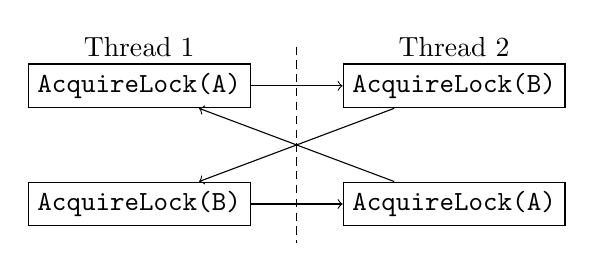
\begin{tikzpicture}
        % \draw (-2,-1) grid (2, 1);
        \node at (-2, 1.5) {Thread $1$};
        \node at (2, 1.5) {Thread $2$};
        \node [rectangle, draw, font=\ttfamily, name=th1_a] at (-2, 1) {AcquireLock(A)};
        \node [rectangle, draw, font=\ttfamily, name=th1_b] at (-2, -0.5) {AcquireLock(B)};
        \node [rectangle, draw, font=\ttfamily, name=th2_b] at (2, 1) {AcquireLock(B)};
        \node [rectangle, draw, font=\ttfamily, name=th2_a] at (2, -0.5) {AcquireLock(A)};
        \draw [->] (th1_a) -- (th2_b);
        \draw [->] (th1_b) -- (th2_a);
        \draw [->] (th2_a) -- (th1_a);
        \draw [->] (th2_b) -- (th1_b);
        \draw [densely dashed] (0, 1.5) -- (0, -1);
    \end{tikzpicture}
    \caption{Deadlock dependency graph.}
    \label{fig:deadlock}
\end{figure}

\subsubsection{System Model}
\begin{itemize}
    \item We have a finite number of resources.
    \item Resources are organized into classes.
    \item Processes compete for accessing resources.
    \item If a process requests an instance of a resource class,
    any instance of that class must satisfy the process.
\end{itemize}

\subsubsection{Resource Usage Protocol}
\begin{itemize}
    \item \textbf{Request} - the process either gets an instance of the resource immediately or waits until one is available.
    \item \textbf{Use} - the process can operate on its resource instance.
    \item \textbf{Release} - the process releases its resource instance.
\end{itemize}

\subsubsection{Deadlock Definition}
\paragraph{Informal Definition}
A set of two or more processes are deadlocked if:
\begin{itemize}
    \item They are blocked.
    \item Each is holding a resource.
    \item Each is waiting to acquire a resource held by another process in the set.
\end{itemize}
\paragraph{Formal Definition}
In a formal way the conditions necessary for a deadlock are the following:
\begin{itemize}
    \item \textbf{Mutual Exclusion} - only one process can use a resource at a time.
    \item \textbf{Hold \& Wait} - a process holding at least one resource is waiting to acquire additional resources which are currently held by other processes.
    \item \textbf{No Preemption} - a resource can only be released voluntarily by the process holding it.
    \item \textbf{Circular Wait} - a cycle of process requests exists ($P_0 \rightarrow P_1 \rightarrow \dots P_{n-1} \rightarrow P_0$).
\end{itemize}

\subsubsection{Deadlock Prevention}
Restrict the way requests can be made.

\paragraph{Mutual Exclusion}
Not required for shared resources, however it must hold for non-shareable files.

\paragraph{Hold \& Wait}
Must guarantee that whenever a process requests a resource, it does not hold any other resources.
Require the process to request and allocate all its resources before it begins execution.
Low resource utilization; possibly resulting in starvation.

\paragraph{No Preemption}
If a process that is holding some resources requests another resource that cannot be immediately allocated to it,
then all resources currently being held are released.
Preempted resources are added to the list of resources for which the process is waiting.
Process will be restarted only when it can regain its old resources, as well as the new ones that it is requesting.

\paragraph{Circular Wait}
Impose a total ordering of all resource types, requiring that each process requests resources in an increasing order of enumeration.

\subsubsection{Deadlock Avoidance}

Requires the system to have some additional \textit{à priori} information available.
\begin{itemize}
    \item Requires that each process declare the maximum number of resources of each type that it may need.
    \item The deadlock-avoidance algorithm dynamically examines the resource-allocation state to ensure that there can never be a circular-wait condition.
    \item Resource-allocation state is defined by the number of available and allocated resources and the maximum demands of the processes.
\end{itemize}

\paragraph{Banker's Algorithm}
In the banker's algorithm processes declare their maximum resource usage of each type of resource.
This number should not exceed the total number of resources in the system.
Whenever a process requests resources the system must determine if the allocation of such resources will leave the system in a safe state.
If it does leave the system in a safe state, the resources are allocated, otherwise the process must wait until enough resources are available.

Several data structures are required for the banker's algorithm,
these data structures encode the resource-allocation state.
In the following data structures, $n$ is the number of processes in the system and
$m$ is the number of resource types.
\begin{itemize}
    \item \textbf{Available} - A vector of length $m$ indicates the number of available resources of each type.
    If $\mathbf{Available}[j]$ equals $k$, then $k$ instances of resource type $R_i$ are available.
    \item \textbf{Max} - An $n \times m$ matrix defines the maximum demand of each process.
    If $\mathbf{Max}[i][j]$ equals $k$, then process $P_i$ may request at most $k$ instances of resource type $R_j$.
    \item \textbf{Allocation} - An $n \times m$ matrix defines the number of resources of each type currently allocated to each process.
    If $\mathbf{Allocation}[i][j]$ equals $k$, then process $P_i$ is currently allocated $k$ instances of resource type $R_j$
    \item \textbf{Need} - An $n \times m$ matrix indicates the remaining resource need of each process.
    If $\mathbf{Need}[i][j]$ equals $k$, then process $P_i$ may need $k$ more instances of resource type $R_j$ to complete its task.
    Note that $\mathbf{Need}[i][j] = \mathbf{Max}[i][j] - \mathbf{Allocation}[i][j]$.
\end{itemize}

The \textit{safety check} algorithm works as follows:
\begin{enumerate}
    \item Let \textbf{Work} and \textbf{Finish} be vectors of length $m$ and $n$, respectively.
    Initialize $\mathbf{Work} = \mathbf{Available}$ and $\mathbf{Finish} = false$ for $i = 0, 1, \dots, n - 1$.
    \item Find an index $i$ such that both:
    \begin{enumerate}
        \item $\mathbf{Finish}[i] == false$
        \item $\mathbf{Need}_i \le \mathbf{Work}$
    \end{enumerate}
    If no such $i$ exists, go to step 4.
    \item $\mathbf{Work} = \mathbf{Work} + \mathbf{Allocation}_i$\\
    $\mathbf{Finish}[i] = true$\\
    Go to step 2.
    \item If $\mathbf{Finish}[i] == true$ for all $i$, then the system is in a safe state.
\end{enumerate}

For the \textit{resource requesting} algorithm, let $\mathbf{Request}_i$ be the request vector for process $P_i$.
If $\mathbf{Request}_i [j] == k$, then process $P_i$ wants $k$ instances of resource type $R_j$.
The algorithm then works as follows:
\begin{enumerate}
    \item If $\mathbf{Request}_i \le \mathbf{Need}_i$, go to step 2.
    Otherwise, raise an error condition, since the process has exceeded its maximum claim.
    \item If $\mathbf{Request}_i \le \mathbf{Available}$, go to step 3.
    Otherwise, $P_i$ must wait, since the resources are not available.
    \item Have the system pretend to have allocated the requested resources to process $P_i$ by,
    modifying the state as follows:\\
    $\mathbf{Available} = \mathbf{Available} - \mathbf{Request}_i$\\
    $\mathbf{Allocation}_i = \mathbf{Allocation}_i + \mathbf{Request}_i$\\
    $\mathbf{Need}_i = \mathbf{Need}_i - \mathbf{Request}_i$\\
    If the resulting resource-allocation state if safe,
    the transaction is complete, and process $P_i$ is allocated its resources.
    However, if the new state is unsafe, then $P_i$ must wait for $\mathbf{Request}_i$,
    and the old resource-allocation state is restored.
\end{enumerate}


\bibliography{bibliography} % Use the bibliography.bib file for the bibliography
\bibliographystyle{plainnat} % Use the plainnat style of referencing
\end{document}